% Material suplementario
\section*{Material suplementario}

\subsection{Balance molar de la cámara y conversión a ppm}
\label{sup:balance}
% TODO S1

\subsection{Extensiones del núcleo larvario al régimen por lotes}
\label{sup:extensiones}
% TODO S2

\subsection{Módulo microbiano del lecho: constante efectiva y humedad}
\label{sup:microbiano}
% TODO S3

\subsection{Justificación de las cotas de búsqueda de la calibración}
\label{sup:cotas}
% TODO S4

\subsection{Parámetros fijos y tomados de la literatura}
\label{sup:params}
% TODO S5

\subsection{Dimensiones del montaje y equivalencias de materia seca}
\label{sup:montaje}
% TODO S6

\subsection{Propagación de la incertidumbre de las tasas}
\label{sup:incertidumbre}
% TODO S7

\subsection{Validación externa: digitalización y transferencia de estados}
\label{sup:externa}

Los datos externos se digitalizaron de las figuras de los estudios originales (300 dpi) y se verificaron contra los valores reportados en texto y tablas de cada artículo. La transferencia usa dos niveles. \emph{Nivel A (transferencia pura):} todos los parámetros congelados en los valores canónicos propios, incluido el pastoreo ($\gamma = 0.5798$); el estado inicial se transplanta desde la trayectoria calibrada de D1. \emph{Nivel B (ajuste mínimo):} Ermolaev reajusta solo $(f, t_{p,\min}, \rho, B_{\max,0})$ contra sus tres tasas y su acumulado; Schøn reajusta solo $f$ por dieta contra sus curvas horarias. En ambos niveles el módulo microbiano de D1 ($k_{\mathrm{ref}}$, $\delta_{CS}$), el decaimiento $k_d$ y el módulo de prepupa se transfieren sin reajuste. El CO$_2$ se compara en flujo (mg CO$_2$/min por caja en Ermolaev; mL/min en Schøn), sin conversión de cámara. El Cuadro~\ref{tab:ermolaev-detalle} detalla el ajuste por punto en Ermolaev y la Figura~\ref{fig:externa-ermolaev} muestra las curvas completas.

\begin{table}[htbp]
  \centering
  \small
  \caption{Validación externa con \textcite{ermolaevGreenhouseGasEmissions2019}, tratamiento L: tasas puntuales y acumulado observados (media~$\pm$~DE entre réplicas) frente a los Niveles A y B del modelo.}
  \label{tab:ermolaev-detalle}
  \begin{tabular}{lrrrr}
    \toprule
    Día & Obs (mg/min) & Obs acum (g/kg FW) & Nivel A (mg/min / g/kg) & Nivel B (mg/min / g/kg) \\
    \midrule
    2  & 2.53~$\pm$~1.1 & 9.1  & 5.07 / 6.2   & 2.58 / 4.0 \\
    7  & 8.04~$\pm$~1.6 & 37.3 & 9.37 / 58.6  & 8.05 / 40.9 \\
    11 & 5.58~$\pm$~1.5 & 68.6 & 5.36 / 92.5  & 5.65 / 74.5 \\
    14 & ---            & 92.4~$\pm$~14.5 & 3.67 / 108.9 & 3.87 / 91.9 \\
    \bottomrule
  \end{tabular}
\end{table}

\begin{figure}[htbp]
  \centering
  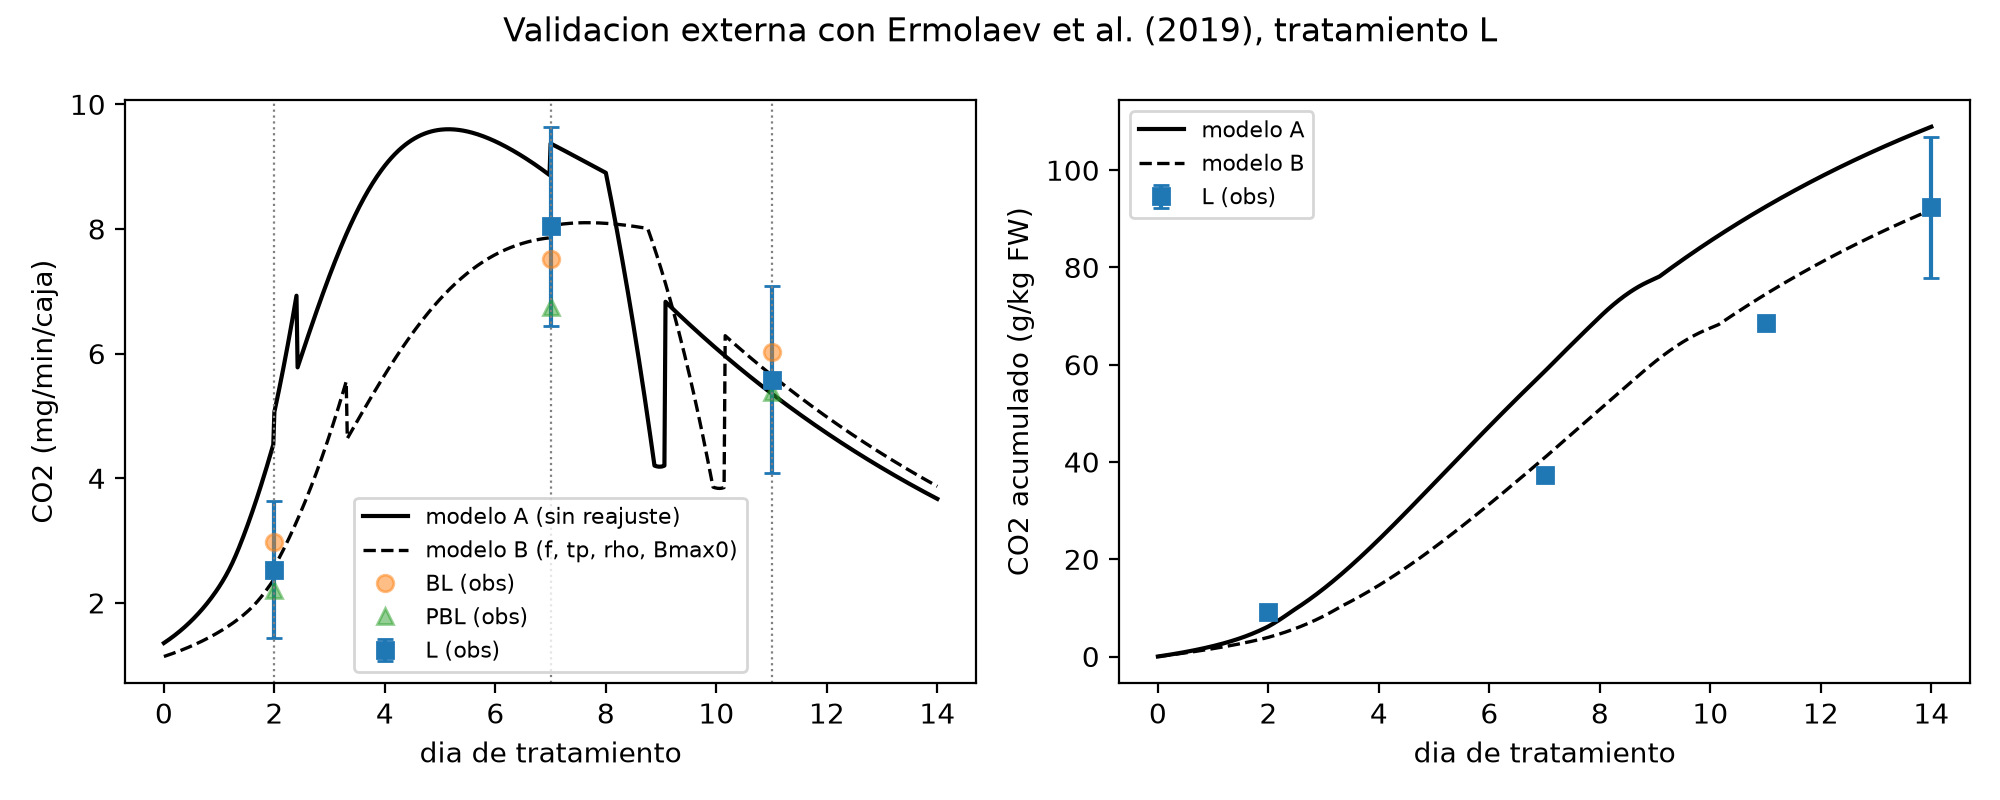
\includegraphics[width=\textwidth]{figuras/validacion_ermolaev.png}
  \caption{Validación externa con \textcite{ermolaevGreenhouseGasEmissions2019}: flujos (izquierda) y acumulado (derecha) del tratamiento L; Niveles A y B del modelo frente a la observación. Las líneas punteadas verticales marcan los días de alimentación.}
  \label{fig:externa-ermolaev}
\end{figure}

\begin{figure}[htbp]
  \centering
  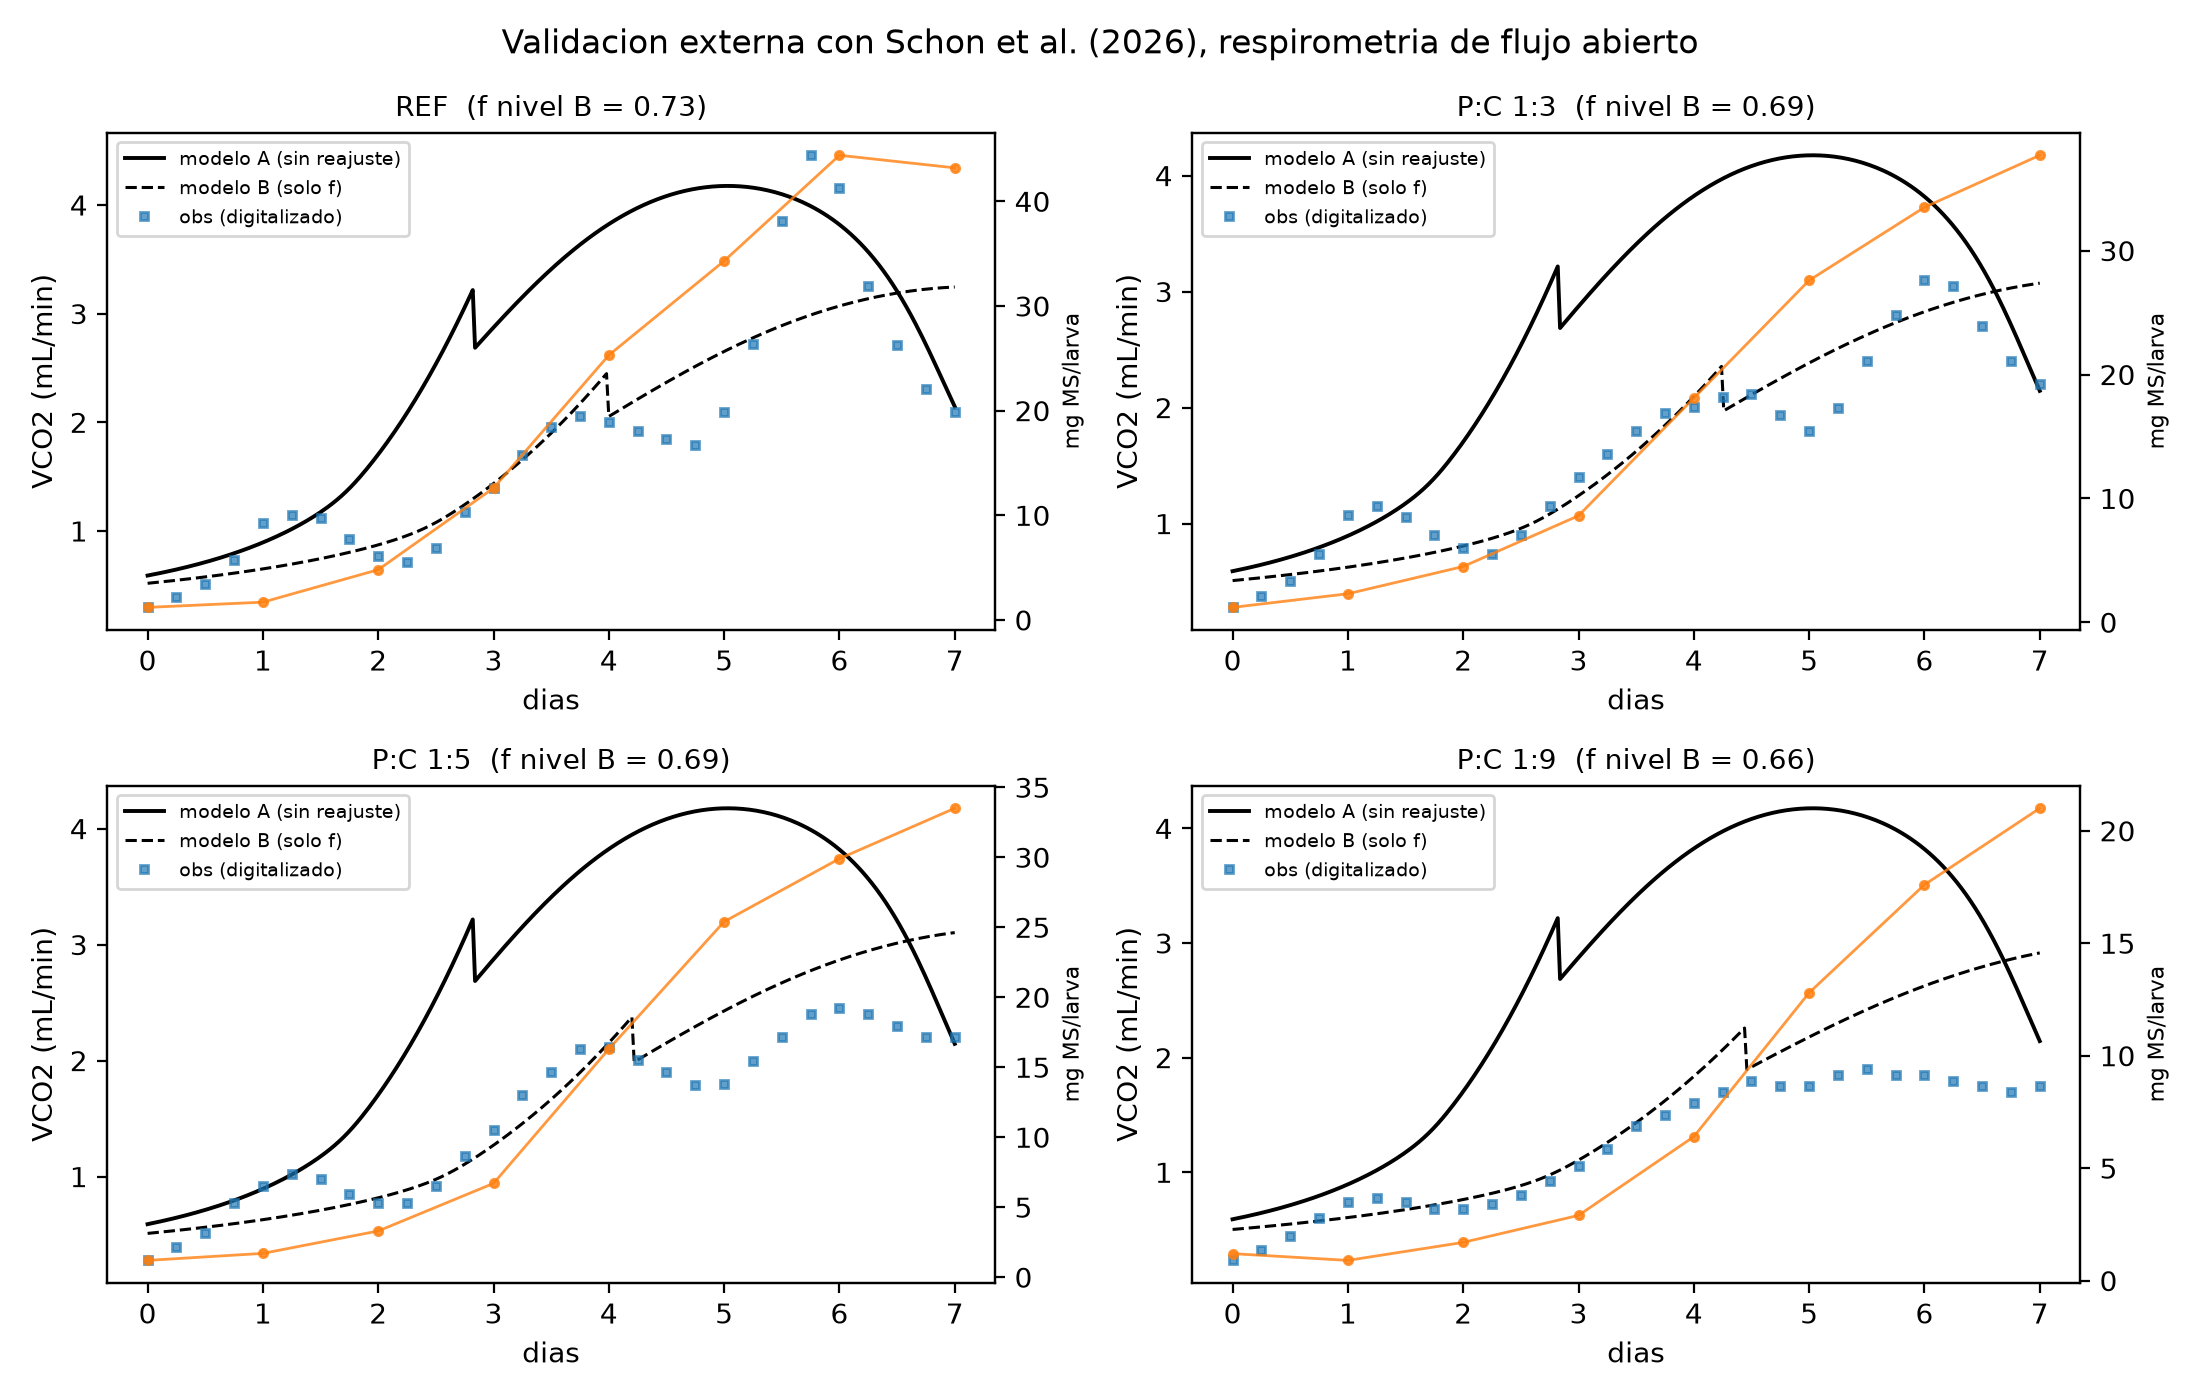
\includegraphics[width=\textwidth]{figuras/validacion_schn.png}
  \caption{Validación externa con \textcite{schonUsingGasExchange2026}: curvas de VCO$_2$ (eje izquierdo) y masa de las larvas (eje derecho, naranja) para las cuatro dietas; Nivel A (línea continua), Nivel B (línea discontinua, con $f$ indicado) y observación digitalizada.}
  \label{fig:externa-schn}
\end{figure}

\subsection{Correspondencia entre el modelo de Eriksen y la implementación}
\label{sup:correspondencia}
% TODO S9: tabla ecuación impresa <-> Excel oficial <-> código
